%! TEX root = ../main.tex
% ==============================================================
% IMMUTABLE — generated automatically, do not edit this block
%
% — Provenance ───────────────────────────────────────────────────
%   script            : analysis_scratch/per40_vs_per240_outin.py
%   computed_in       : analysis_scratch/per40_vs_per240_outin.py (short-run OUT/IN from combined_meta 'IN/OUT Amplitude (FFT)' canonical columns; long-run OUT/IN from H&G [50T, 60T] window via np.fft.fft on interpolated eta)
%   plot_type         : per40_vs_per240_outin
%   data_class        : DFS
%   generated_at      : 2026-04-21T12:10:55
%   findings_doc      : analysis_scratch/per40_vs_per240_outin_findings.md
%
% — Thesis context ──────────────────────────────────────────────
%   chapter           : 04
%   caption_label     : fig:ch04_per40_vs_per240_outin
%   caption_short     : OUT/IN (FFT) at the paddle frequency versus $kL$, split by paddle drive 0.10, 0.20, 0.30\,V (one panel each)
%
% — Filters ────────────────────────────────────────────────────
%   panel             : full
%   wind              : no, full
%   amplitude [V]     : 0.1, 0.2, 0.3
%   frequency [Hz]    : 1.3, 1.6
%   probes            : 
%   run_category      : 
%   quality_flag      : ok+probe_malfunction_secondary
%   mooring           : below_90_loose
%
% — Data provenance ────────────────────────────────────────────
%   n_runs            : 78
%   in_probes_used    : 9373/170+9373/340
%   out_probes_used   : 12400/250
%   probe_configs     : march2026_better_rearranging
%   non_final_config_n: 
%   datasets        :
%     PROCESSED-20260326-ProbePos4_31_FPV_2-tett6roof-under9Mooring-height100-lowrange
%     PROCESSED-20260327-ProbePos4_31_FPV_2-tett6roof-under9Mooring30-height100-lowrange
%   run_paths       :
%     (omitted — aggregate over > threshold runs, see datasets)
%
% — Method / numerical parameters ─────────────────────────────
%   grouper           : per (freq, amp, wind, method) group; n-average with std
%   collapse_panels   : False
%   fft_window_hz     : 0.1
%   extra_params      : HG_MIN_PERIODS=50, HG_window=[50T, 60T], fft_band_hz=0.05, IN_probes=['9373/170', '9373/340'], OUT_probe=12400/250, datasets=['20260326-ProbePos4_31_FPV_2-tett6roof-under9Mooring-height100-lowrange', '20260327-ProbePos4_31_FPV_2-tett6roof-under9Mooring30-height100-lowrange']
%
% — Summary stats cited in caption ────────────────────────────
%   stat:n_short_runs : 35
%   stat:n_long_runs  : 43
%   stat:n_matched_cells : 22
%   stat:delta_OUTIN_median : 0.0106
%   stat:delta_OUTIN_max : 0.0747
%   stat:delta_OUTIN_rel_median_pct : 1.62
%   stat:delta_OUTIN_rel_max_pct : 10.7
%   stat:HG_min_periods : 50
%   stat:HG_window_periods : [50T, 60T]
%
% — Subfigures available ───────────────────────────────────────
%     FIGURES/ch04_per40_vs_per240_outin.pdf
% ── end immutable block ─────────────────────────────────────────
\begin{figure}[htbp]
  \centering
  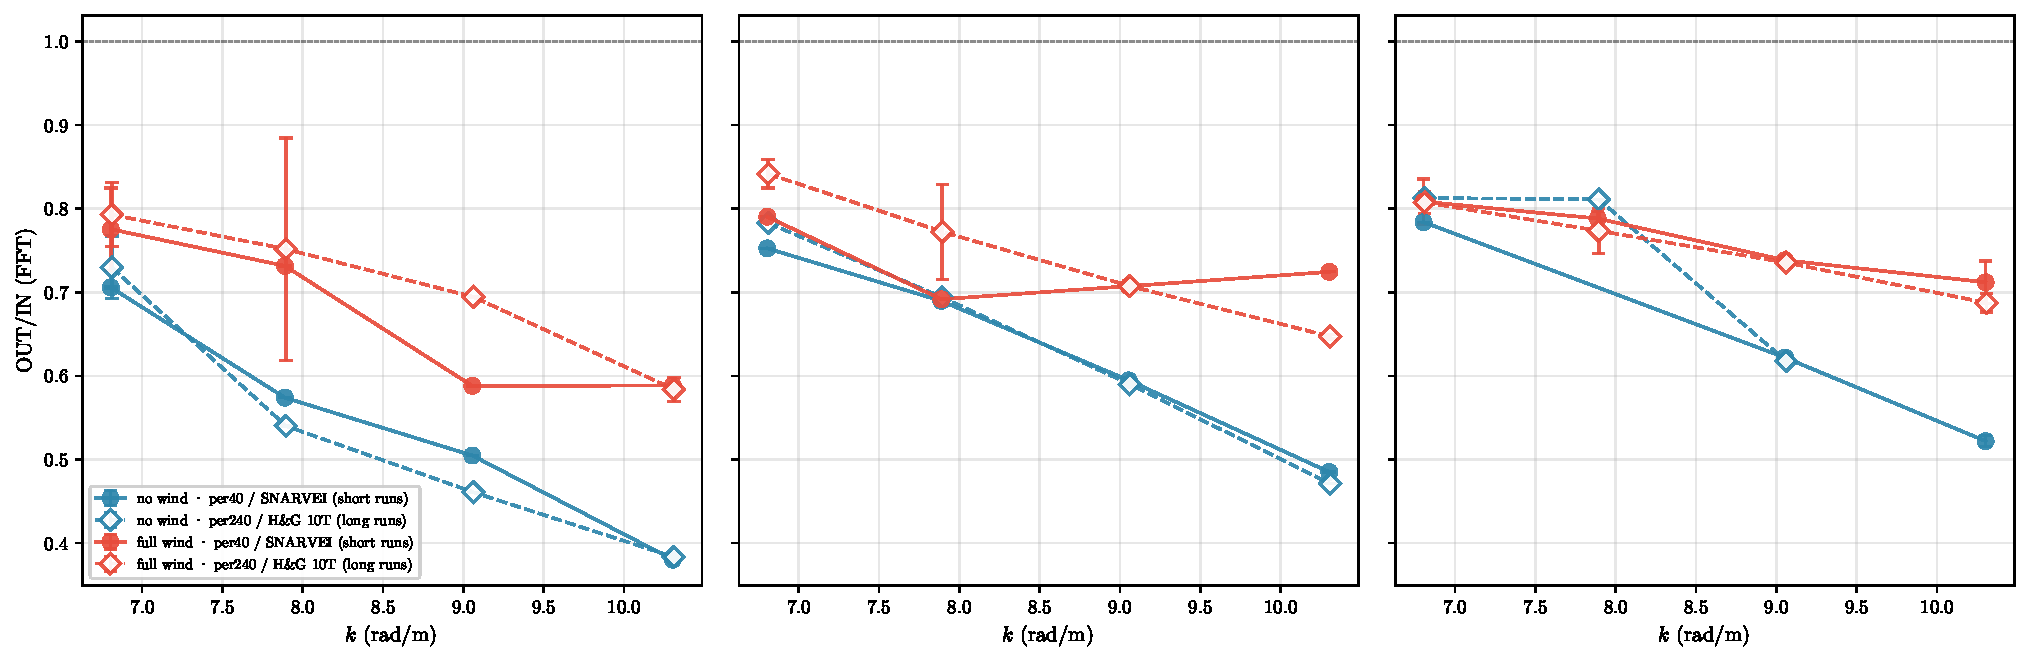
\includegraphics[width=\linewidth]{FIGURES/ch04_per40_vs_per240_outin.pdf}
  \caption[OUT/IN (FFT) at the paddle frequency versus $kL$, split by paddle drive 0]{
    OUT/IN (FFT) at the paddle frequency versus $kL$, split by paddle drive 0.10, 0.20, 0.30\,V (one panel each). Two analysis-window methods per condition: pipeline SNARVEI window applied to short runs ($N_\mathrm{input\_periods} < 50$; filled circles), Huseby--Grue 10T window $t \in [50T, 60T]$ from wavemaker start applied to long runs (open diamonds). Blue: no wind; red: full wind. Error bars: run-to-run standard deviation within each (frequency, amplitude, wind, method) cell. Canonical IN amplitude is the mean of parallel probes 9373/170 and 9373/340; OUT amplitude is from 12400/250 (both via the same FFT peak-bin convention). Dataset: cond4 low-range, mooring \texttt{below\_90\_loose} (230+300 merged), quality flag $\in$ \{ok, probe\_malfunction\_secondary\}.
  }
  \label{fig:ch04_per40_vs_per240_outin}
\end{figure}
